\chapter{Evaluation} 

\label{Chapter5}

\lhead{Chapter 5. Evaluation} 

\section{FFmpeg experiment design and benchmark}

\begin{figure}[!htbp]
	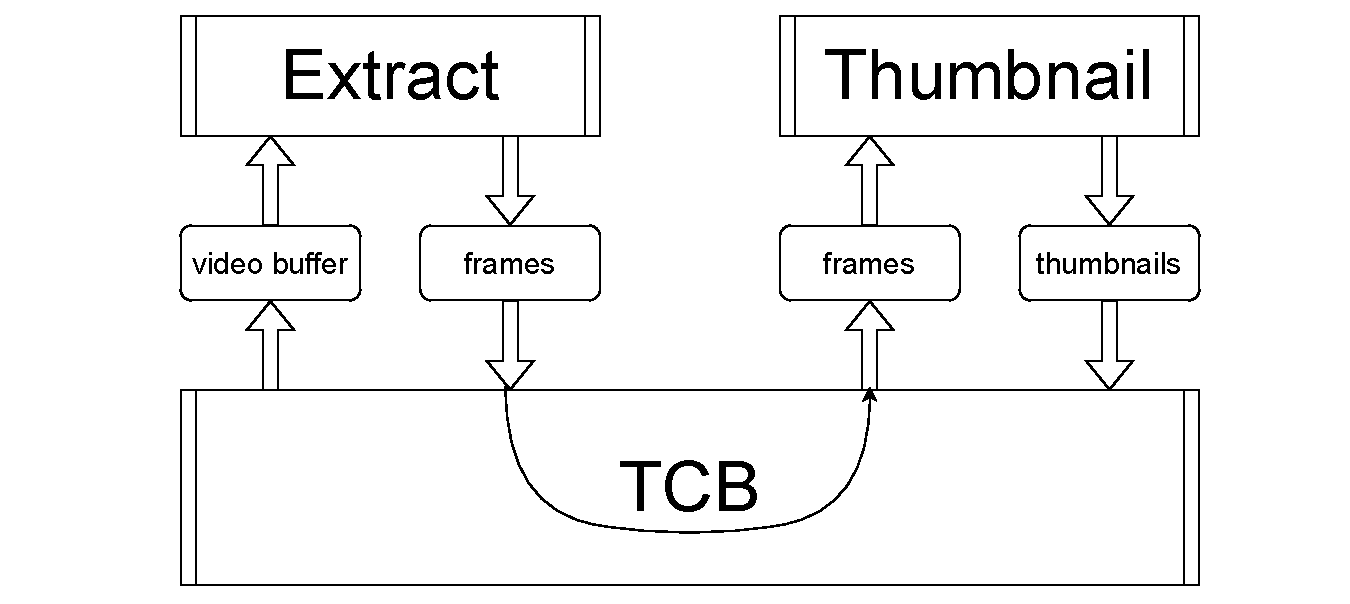
\includegraphics[width=1.0\columnwidth]{figures/ffmpeg-pinpeline.pdf}
\caption{Overhead of FFmpeg (ARM)}
	\label{fig:ffmpeg-arm}
%\vspace{-5mm}
\end{figure}

\begin{figure}[!htbp]
	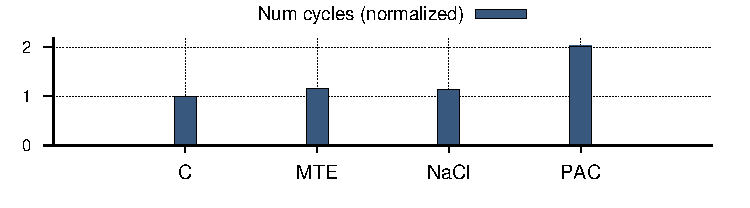
\includegraphics[width=1.0\columnwidth]{figures/ffmpeg-arm.pdf}
\caption{Overhead of FFmpeg (ARM)}
	\label{fig:ffmpeg-arm}
%\vspace{-5mm}
\end{figure}

\begin{figure}[!htbp]
	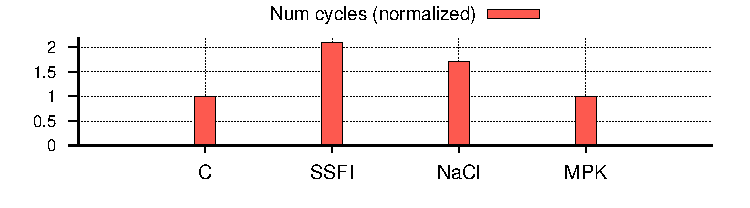
\includegraphics[width=1.0\columnwidth]{figures/ffmpeg-x86.pdf}
\caption{Overhead of FFmpeg (x86)}
	\label{fig:ffmpeg-x86}
%\vspace{-5mm}
\end{figure}

\section{Microarchitectural comparison}

\begin{table}[!htbp]
    \begin{small}
    \begin{center}
  \begin{tabular}{| l | c | c | c | c | c |}
  \hline
  (in Millions)    & C   & SSFI   & NaCl & MPK   \\
  \hline
  \hline
  Cycles           & 5995 & 11578  & 10188 & 5996  \\
  Instructions     & 14681  & 34797  & 25846 & 14681 \\
  Branches         & 905   & 938   & 907  & 905   \\
  Branches mispred & 60   & 63    & 56   & 60    \\
  loads            & 3267  & 3844  & 3448 & 3267  \\
  stores           & 1415  & 1594   & 1493  & 1415   \\
  \hline
  \end{tabular}
  \end{center}
\end{small}
  \caption{Microarchitectural comparison of SFI and C on FFmpeg-x86 benchmark.}
  \label{table:micro-ffmpeg-x86}
  \end{table}


%tirth here if you want to disable arm numbers
%\iffalse
\begin{table}[!htbp]
    \begin{small}
    \begin{center}
  \begin{tabular}{| l | c | c | c | c | c |}
  \hline
  (in Millions)    & C   & MTE   & NaCl & PAC   \\
  \hline
  \hline
  Cycles           & 2253 & 2712  & 2673 & 4689  \\
  Instructions     & 7487  & 7487  & 7327 & 14180 \\
  Branches         & 407   & 427   & 419  & 426   \\
  Branches mispred & 104   & 22    & 22   & 21    \\
  loads            & 1489  & 1504  & 1465 & 3288  \\
  stores           & 619  & 618   & 610  & 811   \\
  \hline
  \end{tabular}
  \end{center}
\end{small}
  \caption{Microarchitectural comparison of SFI and C on FFmpeg-AArch64 benchmark.}
  \label{table:micro-ffmpeg-arm}
  \end{table}
%\fi